\chapter{Compute e Virtualizzazione}

\section{Architettura Compute: CPU, GPU e NPU}
L'elaborazione dei dati (Compute) è il terzo pilastro del datacenter. L'evoluzione hardware moderna è guidata dalla fine della scalabilità lineare del singolo core (Legge di Moore) e dalla necessità di efficienza e specializzazione per carichi di lavoro legati all'Intelligenza Artificiale.

\subsection{Sostenibilità Energetica}
I datacenter consumano enormi quantità di energia elettrica e acqua. Le metriche di riferimento sono:
\begin{itemize}
    \item \textbf{PUE (Power Usage Effectiveness):} Rapporto tra energia totale consumata dal datacenter e quella effettivamente usata dai server. Il valore ideale è 1.0.
    \item \textbf{WUE (Water Usage Effectiveness):} Consumo idrico per kWh, critico nei datacenter che usano raffreddamento evaporativo (Torri di raffreddamento).
\end{itemize}

\subsection{Architettura CPU: Pipeline e Multi-Core}
Storicamente, per aumentare le prestazioni, si aumentava la frequenza di clock e si ottimizzava la \textbf{Pipeline delle istruzioni} (suddivisa classicamente nelle fasi: \textit{Instruction Fetch, Decode, Execute, Memory Access, Write-back}). Aumentando la profondità della pipeline (fino a 20+ stadi), si potevano eseguire più istruzioni sovrapposte nel tempo, ma gli errori di previsione dei salti (\textit{Branch Misprediction}) causavano lo stallo e lo svuotamento completo della coda ("bolle" nella pipeline), vanificando l'efficienza. 

Arrivati al limite fisico del calore dissipabile (Power Wall), si è passati al parallelismo Multi-Core. Per superare i colli di bottiglia della condivisione della RAM, le CPU moderne adottano architetture \textbf{NUMA (Non-Uniform Memory Access)}, in cui ogni processore ha un proprio banco di memoria locale ad accesso diretto rapido; l'accesso alla RAM degli altri processori avviene tramite interconnessioni esterne a latenza maggiore.

\textbf{Hyperthreading e SMT (Simultaneous Multithreading)}\\
Per ridurre al minimo i tempi morti (idle time) in cui un core attende dati dalla memoria, i progettisti hanno introdotto l'\textbf{Hyperthreading} (o SMT). Il trucco consiste nel duplicare solo le risorse "leggere" (come i registri e il program counter), mantenendo condivise le costose unità di calcolo fisico (ALU). Il sistema operativo vede \textbf{due core logici} per ogni core fisico: quando un thread è in stallo per un \textit{cache miss}, il core scambia istantaneamente contesto ed esegue le istruzioni dell'altro thread.
Sebbene eccellente per server web e database ad alto I/O, l'HT è \textbf{dannoso in ambito HPC} (High Performance Computing): se due thread devono fare calcolo intensivo matematico simultaneo, lotteranno aspramente per l'unica ALU condivisa, riducendo le performance generali. Nei supercomputer l'HT viene perciò disabilitato.

\begin{tipbox}[Overbooking e Memory Ballooning]
La virtualizzazione si fonda sull'\textbf{Overbooking} (sovra-allocazione logica delle risorse fisiche sottostanti). Oltre all'ovvio over-commit delle vCPU, si esegue overbooking pesante sulla RAM. Un meccanismo chiave è il \textbf{Memory Ballooning}: l'hypervisor inietta un driver-palloncino nel kernel del SO ospite. Se il server fisico sta esaurendo la vera RAM, l'hypervisor "gonfia" il palloncino. Il SO ospite crede di aver bisogno urgentemente di memoria interna, swappa i propri processi meno usati sul suo disco virtuale e restituisce la RAM vera al palloncino (e quindi all'hypervisor). L'hypervisor maschera inoltre enormi quantità di RAM tramite \textit{Memory Page Sharing} (es. KSM deduplica le pagine di sistema operativo identiche tra decine di VM Windows uguali).
\end{tipbox}

\begin{warningbox}[Vulnerabilità Side-Channel]
Condividere fisicamente la cache L1 e i buffer di esecuzione tra due thread apre la porta ad attacchi speculativi come \textbf{Spectre} o \textit{MDS}. Un thread malevolo può dedurre dati segreti del thread "fratello" misurando la latenza della cache. Per massima sicurezza, alcuni cloud provider disabilitano del tutto l'SMT.
\end{warningbox}

\begin{figure}[H]
    \centering
    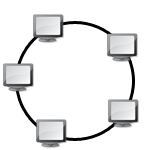
\includegraphics[width=0.6\textwidth]{images/ring_topology.png}
    \caption{Schema logico di una topologia Ring, storicamente usata per l'interconnessione interna dei core CPU.}
\end{figure}
\textbf{Interconnessione interna: Crossbar vs Bus}\\
A livello di interconnessione interna (die), le prime CPU multi-core usavano un \textit{Bus Condiviso}, che diventava subito un collo di bottiglia: solo un core alla volta poteva parlare. Oggi si utilizza la \textbf{Crossbar} (o una \textit{Mesh Network}): una matrice di interconnessione che permette a molteplici core di comunicare simultaneamente con banchi di memoria o I/O diversi senza intralciarsi, garantendo \textit{bisection bandwidth} completa.

Questo approccio reticolare si sposa perfettamente con l'architettura a \textbf{Tile (o Chiplet)}: i processori moderni non sono più un unico monolite di silicio prono a difetti, ma un mosaico di piccoli chip iperspecializzati (Compute Tile, I/O Tile) stampati con nodi differenti e incollati sullo stesso package, migliorando enormemente le rese produttive (yield) e abbassando i costi. Esempi concreti di questo approccio sono il fabric di interconnessione \textbf{AMD Infinity Fabric} per unire i chiplet nei processori EPYC, e le tecnologie di packaging avanzato 3D come \textbf{Intel EMIB e Foveros} (usate nelle architetture Meteor Lake e Sapphire Rapids) che impilano i die di silicio verticalmente.

\subsection{GPU e NPU: Il cambio di paradigma}
\begin{itemize}
    \item \textbf{CPU:} Ottimizzata per la \textit{minima latenza}. Pochi core molto complessi con esecuzione \textit{Out-of-Order} e grandi cache.
    \item \textbf{GPU:} Ottimizzata per il \textit{massimo throughput}. Migliaia di core semplici che eseguono lo stesso calcolo in parallelo (SIMT), ideale per l'addestramento dell'AI.
    \item \textbf{NPU (Neural Processing Unit):} Circuiti dedicati e specializzati esclusivamente nel calcolo tensoriale e inferenza AI a bassa precisione numerica e bassissimo consumo energetico.
\end{itemize}

\section{Architetture Server Fisici e BMC}
L'involucro fisico (form factor) dei server si è diversificato negli anni per rispondere a diverse esigenze di densità, potenza di calcolo e dissipazione termica.

\subsection{Server Rack (1U / 2U)}
\begin{figure}[H]
    \centering
    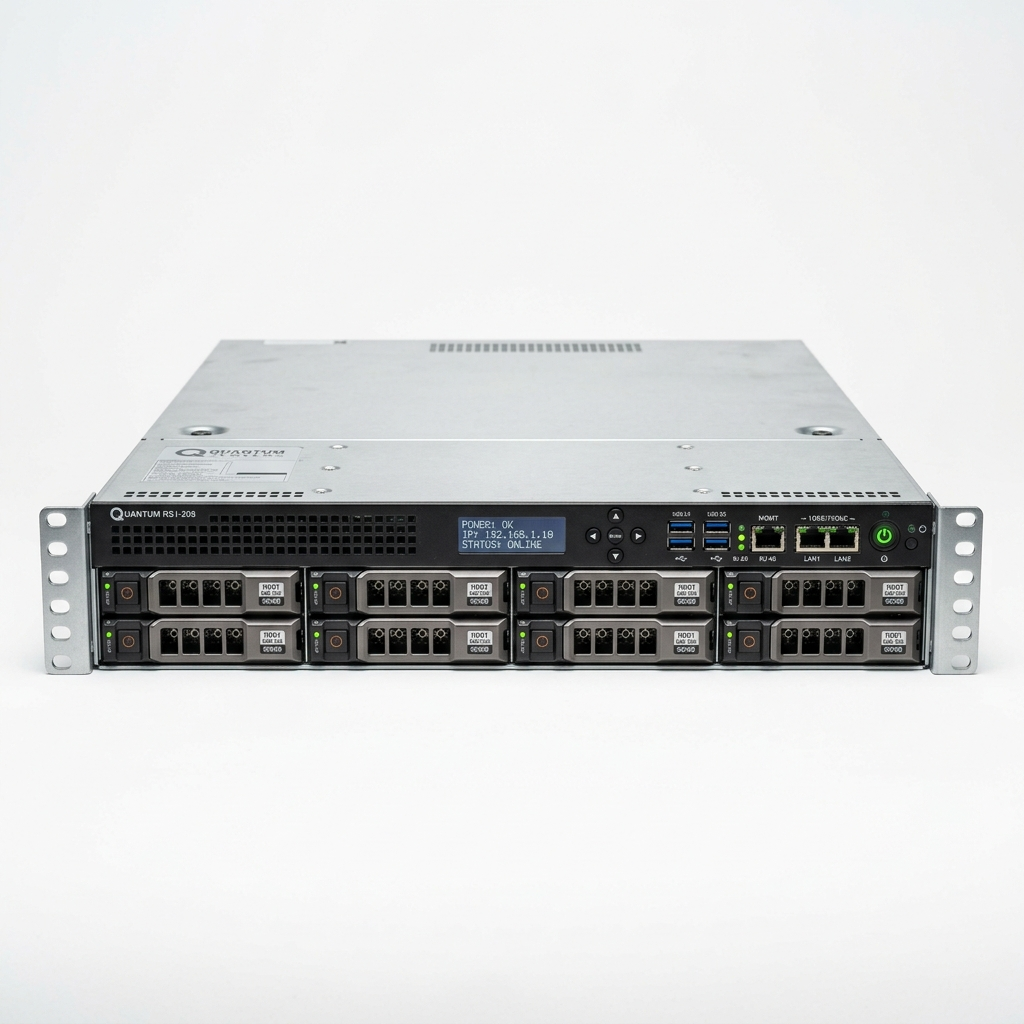
\includegraphics[width=0.7\textwidth]{images/rack_server_1u.png}
    \caption{Server Rack 1U standard con alloggiamenti per dischi frontali (hot-swap).}
\end{figure}
È il formato "general-purpose" più diffuso nei data center tradizionali. Un server rack è un computer completo e indipendente (dotato di propri alimentatori, ventole, CPU, RAM e dischi) racchiuso in uno chassis metallico standardizzato largo 19 pollici. L'altezza si misura in unità rack (U, circa 4,4 cm). Sono ideali per workload eterogenei, ma in grandi quantità richiedono un enorme lavoro di cablaggio singolo per ogni macchina (cavi di alimentazione e di rete separati per ogni singolo server).

\subsection{Blade Server}
\begin{figure}[H]
    \centering
    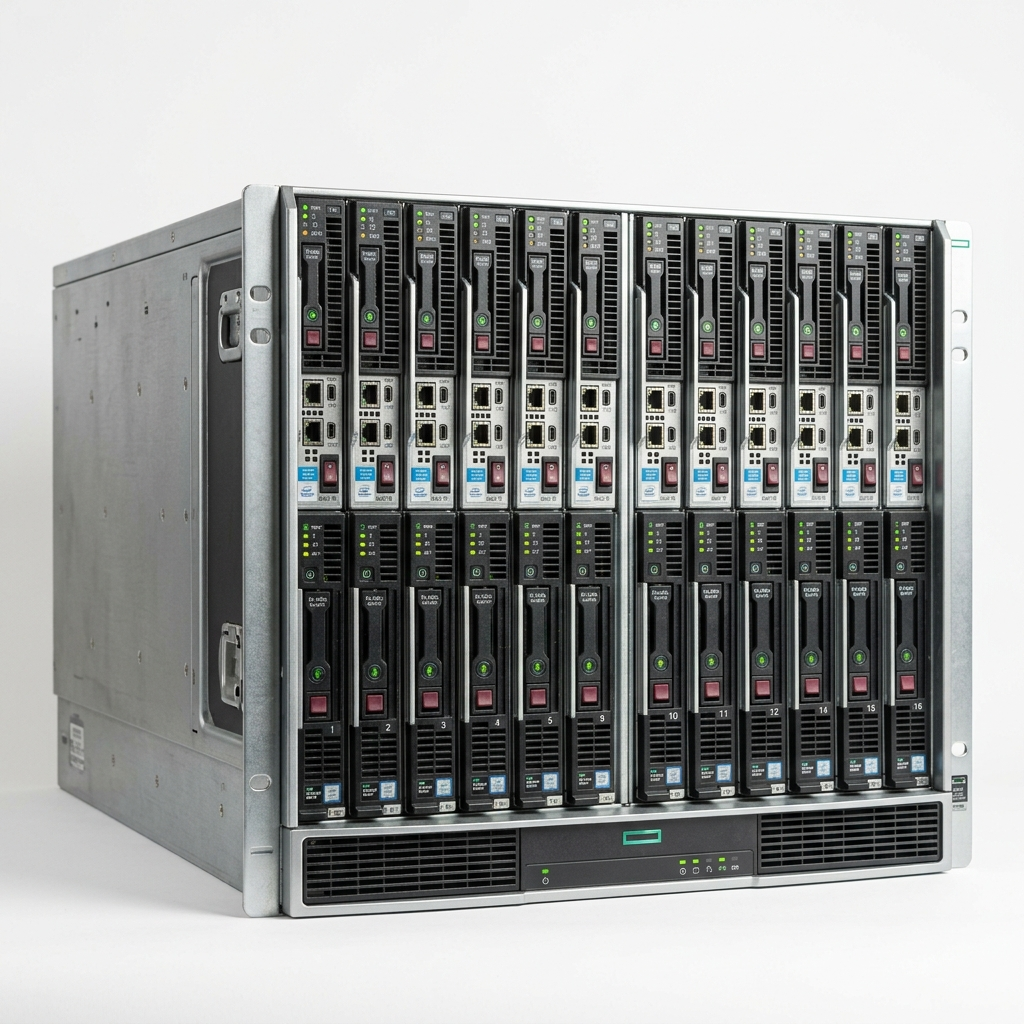
\includegraphics[width=0.7\textwidth]{images/blade_server.png}
    \caption{Chassis Blade System: decine di server-lama inseriti in un singolo modulo.}
\end{figure}
Progettati per ottenere l'altissima densità necessaria nei cluster di virtualizzazione. Un sistema Blade si divide in due componenti: lo \textbf{Chassis} (l'involucro esterno che fornisce alimentazione condivisa, mega-ventole e switch di rete integrati) e le \textbf{Lame} (i server veri e propri). La lama (Blade) è sottilissima perché contiene solo CPU, RAM e pochi dischi; non ha ventole o alimentatori propri. Inserendola nello chassis, si collega automaticamente al \textit{midplane} posteriore, azzerando quasi totalmente il disordine del cablaggio nel rack.

\subsection{Server HGX (AI GPU Server)}
\begin{figure}[H]
    \centering
    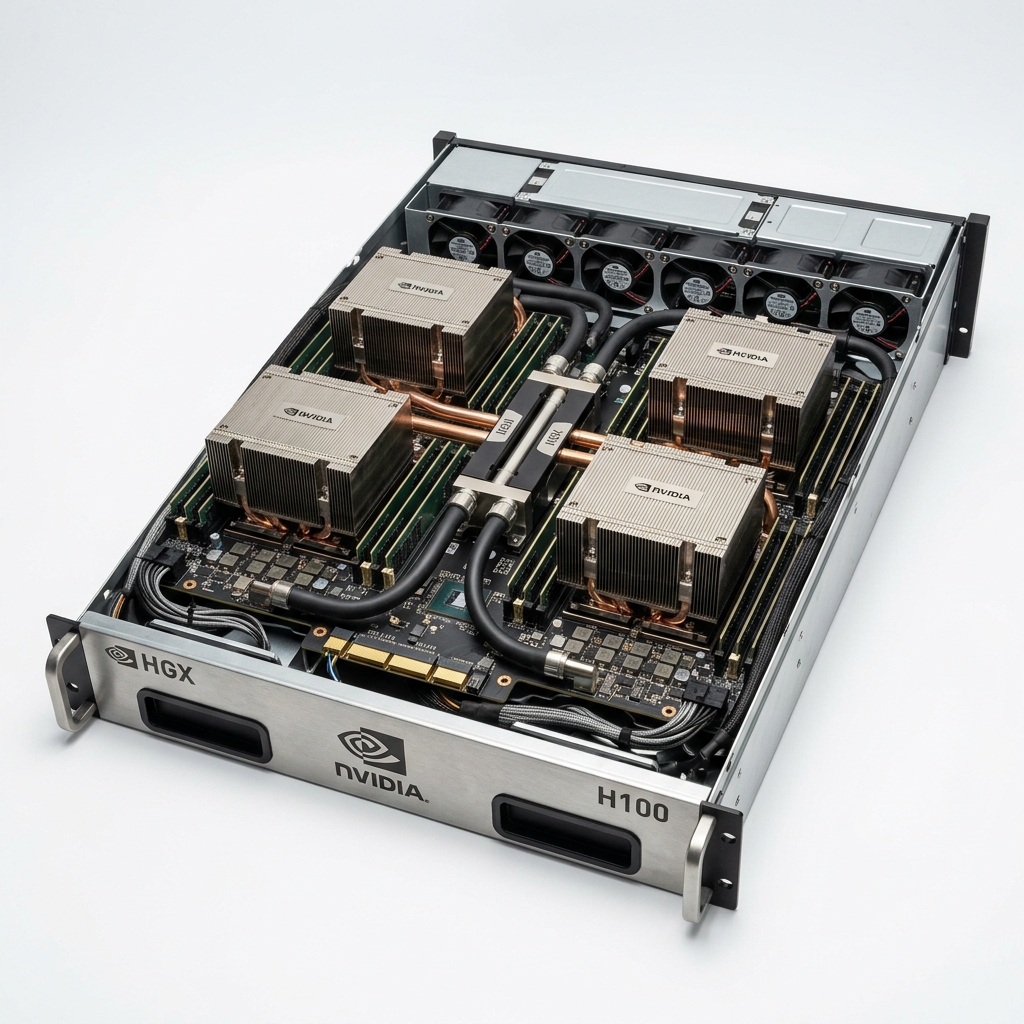
\includegraphics[width=0.7\textwidth]{images/hgx_gpu_server.png}
    \caption{Server HGX (aperto): GPU ad alte prestazioni coperte da enormi dissipatori metallici per gestire il calore estremo.}
\end{figure}
Con l'esplosione dell'intelligenza artificiale generativa, i normali server rack non sono più sufficienti. Un server HGX è una macchina immensa (spesso 4U o 8U, pesante oltre 100 kg) progettata esclusivamente attorno alle GPU (es. NVIDIA H100). Le GPU non sono più inserite come schede PCIe estraibili, ma sono saldate direttamente su una \textit{baseboard} proprietaria e interconnesse tramite bus dedicati (come NVLink) che scavalcano il collo di bottiglia del PCIe. Generano un calore spaventoso, rendendo spesso obbligatorio il passaggio al raffreddamento a liquido (\textit{Direct-to-Chip Liquid Cooling}).

\subsection{Standardizzazione Hyperscaler: Open Compute Project (OCP)}
Creato originariamente da Meta (Facebook) nel 2011, l'\textbf{OCP (Open Compute Project)} è un consorzio no-profit che pubblica le specifiche hardware open source per server e rack da datacenter. L'idea nasce da un'esigenza economica: i server tradizionali di brand contengono molte funzionalità estetiche o di gestione (frontalini in plastica, display, alimentatori ridondati per singolo server) inutili su scala hyperscaler.
Le specifiche OCP definiscono macchine essenziali (spesso prodotte direttamente da costruttori ODM taiwanesi come Quanta o Foxconn), permettendo risparmi enormi. Un'innovazione chiave dell'OCP è il design del rack: l'alimentazione non viene convertita in ogni singolo server, ma centralizzata a monte nel rack e distribuita ai server tramite busbar a 12V o 48V, aumentando l'efficienza energetica e la densità.

\begin{tipbox}[BMC (Baseboard Management Controller) e lo Standard Redfish]
Tutti i server di livello enterprise montano un \textbf{BMC} (es. iLO di HPE o iDRAC di Dell). Si tratta di un micro-computer indipendente inserito nella scheda madre, dotato di una porta di rete dedicata (\textit{out-of-band management}). Essendo alimentato separatamente, permette il controllo fisico del server (accensione, configurazione BIOS, console KVM virtuale) anche se il sistema operativo principale è bloccato o se il server è fisicamente spento.

\textbf{Redfish: L'API del Datacenter Moderno}\\
Storicamente, i BMC venivano gestiti tramite il protocollo IPMI, che col tempo si è rivelato insicuro e difficile da integrare. Per questo motivo, il consorzio DMTF ha introdotto \textbf{Redfish}, lo standard moderno per la gestione dell'infrastruttura.
\begin{itemize}
    \item \textbf{Come funziona:} Redfish espone tutti i parametri hardware tramite una \textbf{RESTful API} standard. Utilizza i protocolli del web moderno (HTTPS per la sicurezza) e restituisce i dati in formato \textbf{JSON} (OData), facilmente leggibile sia dagli umani che dagli script.
    \item \textbf{Cosa fa:} Permette di automatizzare su larga scala le operazioni più tediose. Tramite semplici script Python o strumenti come Ansible, si possono inviare richieste web (GET, POST, PATCH) per monitorare le temperature, aggiornare i firmware, modificare l'ordine di boot o riavviare un intero rack di server, indipendentemente dalla marca dell'hardware sottostante.
\end{itemize}
\end{tipbox}

\section{Virtualizzazione e Live Migration}
La virtualizzazione svincola il software dall'hardware fisico, permettendo a più Sistemi Operativi (Guest) di girare simultaneamente sullo stesso server fisico (Host). Il cuore di questo processo è l'\textbf{Hypervisor} (o Virtual Machine Monitor).

\subsection{L'Evoluzione dell'Hypervisor: Dai Ring CPU alla Virtualizzazione Hardware}
L'architettura x86 originale non era progettata per essere virtualizzata. Prevedeva quattro livelli di privilegio logici chiamati \textbf{Ring}, da Ring 0 (massimo privilegio, destinato al kernel del SO) a Ring 3 (spazio utente). 
In un ambiente virtualizzato, l'Hypervisor deve avere il controllo assoluto, quindi deve risiedere in Ring 0. Questo costringeva i sistemi operativi Guest a scalare in Ring 1 (modalità non privilegiata, definita \textit{Ring De-privileging}). Poiché i SO Guest non sapevano di essere virtualizzati, tentavano di eseguire istruzioni privilegiate (es. manipolazione hardware) che, fallendo, venivano intrappolate dall'Hypervisor. Quest'ultimo doveva tradurle ed emularle in tempo reale (tecnica della \textbf{Binary Translation}), causando un enorme e insostenibile overhead prestazionale.

Il problema è stato risolto nel 2005 dai produttori di CPU con l'introduzione di estensioni hardware dedicate (\textbf{Intel VT-x} e \textbf{AMD-V}). Queste istruzioni hanno creato un nuovo livello di privilegio inferiore allo zero (spesso chiamato colloquialmente \textbf{Ring -1}). Oggi l'Hypervisor risiede in Ring -1, permettendo ai kernel dei sistemi operativi Guest di operare nel loro nativo Ring 0, eseguendo istruzioni in modo diretto e a velocità hardware, annullando la necessità di lenta traduzione binaria.

\subsection{Astrazione dell'Hardware: vCPU, Pause e Resume}
La macchina virtuale non vede la reale CPU fisica, ma una \textbf{vCPU} (Virtual CPU) configurata dall'hypervisor. Questo è un dettaglio cruciale per la portabilità: l'hypervisor può nascondere set di istruzioni troppo recenti (es. AVX-512) mascherando le reali capacità del processore fisico, in modo da poter migrare liberamente la VM anche verso un server più vecchio che non possiede quelle istruzioni. 

Inoltre, siccome l'intero ambiente Guest è solo software in esecuzione su un ciclo \textit{fetch-execute} controllato, l'hypervisor gode del potere di \textbf{Pause and Resume}. Può congelare istantaneamente il sistema operativo salvando \textit{lo stato completo della VM} (registri della CPU, stato della memoria e disco virtuale). Il SO virtualizzato non si accorgerà di nulla, per lui il tempo si sarà semplicemente fermato. 
Tramite gli \textbf{Integration Services}, l'hypervisor forza poi la sincronizzazione del clock alla ripresa (vitale per protocolli come Kerberos che falliscono se l'orario si disallinea), invia segnali di \textit{heartbeat} per capire se il kernel Guest è crashato, e orchestra spegnimenti puliti (graceful shutdown).

\begin{tipbox}[Windows Dual Boot e Secure World con WSL2]
Oggi la virtualizzazione è pervasiva anche sui dispositivi client. All'avvio, un PC con Windows moderno (VBS abilitato) non fa un normale avvio nudo, ma lancia un hypervisor (Hyper-V) che istanzia due ambienti. Il primo è un micro-OS nascosto (\textbf{Secure World}) che isola l'hardware crittografico (es. chiavi BitLocker). Subito dopo viene lanciato l'ambiente Windows desktop principale, che gira quindi \textit{virtualizzato}. Anche se un hacker ottiene i privilegi massimi (Ring 0) sul kernel di Windows, non potrà mai rubare le chiavi crittografiche del Secure World.
Lo stesso hypervisor client trasparente rende possibile \textbf{WSL2} (Windows Subsystem for Linux), che esegue un vero kernel Linux completo in una micro-VM ultraleggera parallelamente a Windows.
\end{tipbox}

\subsection{Il Virtual Switch (vSwitch)}
Per connettere le VM al mondo esterno, l'Hypervisor implementa un \textbf{Virtual Switch} in memoria RAM. Le macchine virtuali possiedono schede di rete logiche (\textbf{vNIC}), che si collegano alle porte del vSwitch. A sua volta, il vSwitch instrada il traffico verso la rete fisica tramite le schede di rete reali del server (\textbf{pNIC}). Il vSwitch gestisce in software logiche complesse come tagging VLAN, traffic shaping e raggruppamento delle interfacce fisiche in modo del tutto trasparente per le macchine virtuali ospiti.

\subsection{Live Migration}
La funzionalità più dirompente della virtualizzazione è la \textbf{Live Migration} (es. VMware vMotion), che permette di spostare una VM accesa da un host fisico a un altro senza interruzione di servizio.
Si sviluppa rigorosamente in tre fasi sequenziali:
\begin{enumerate}
    \item \textbf{Pre-copy (Dirty tracking):} Trasferimento massivo iniziale della memoria mentre la VM gira sul vecchio host. Il sistema traccia attivamente tramite una bitmap (\textit{dirty page tracking}) quali pagine di memoria vengono modificate durante la lenta operazione di copia in rete. Questo ciclo viene ripetuto per trasferire i delta successivi.
    \item \textbf{Stop and copy:} Quando le dirty pages rimaste sono pochissime, la VM viene "congelata" (pausa impercettibile di pochi ms). Viene copiato lo stato residuo dei registri CPU, i buffer di I/O, e la RAM residua. L'esecuzione viene trasferita all'hypervisor di destinazione.
    \item \textbf{Gestione della Rete (Gratuitous ARP):} Poiché il MAC address della VM si è spostato fisicamente su un'altra porta dello switch core del datacenter, il vSwitch di destinazione lancia un \textbf{Gratuitous ARP} broadcast. Questo aggiorna istantaneamente le tabelle CAM di tutti gli switch fisici, garantendo che i pacchetti in transito non vengano persi.
\end{enumerate}

\section{Containerizzazione}
A differenza della virtualizzazione, i \textbf{Container} non emulano un intero hardware o un intero kernel, ma \textbf{condividono il kernel Linux dell'host}. Questo riduce a zero l'overhead, ma cambia radicalmente le modalità di sicurezza e funzionamento in rete.

\subsection{Meccanismi di Isolamento e Vulnerabilità}
L'isolamento, vitale per impedire che i container collassino tra loro, è delegato al kernel del sistema operativo tramite due primitive:
\begin{itemize}
    \item \textbf{Namespaces:} Isolano la visibilità logica. Un namespace fa credere al container di essere l'unico sistema, dotandolo di un PID tree autonomo e mount point esclusivi.
    \item \textbf{Cgroups (Control Groups):} Limitano l'utilizzo hardware (impongono tetti massimi di CPU o ferrei \textit{OOM killer} per la RAM).
\end{itemize}

Condividere il kernel comporta però che una falla in esso colpisca tutti simultaneamente. Il corso cita l'anomalo caso della vulnerabilità \textbf{CVE-2026-31431 ("Copy Fail")} nel modulo \texttt{authencesn}: abusando del \textit{page cache} condiviso tra container, un banale script Python permette non solo la scalata di privilegi, ma un catastrofico \textit{container escape}, mettendo a repentaglio interi nodi di orchestrazione.

\subsection{Dettagli Architetturali Docker}
\begin{itemize}
    \item \textbf{Overlay File System:} I container usano file system a strati (es. \textit{overlay fs}). L'immagine del container è immutabile (sola lettura). Avviandolo, si crea un leggero layer \textit{Read-Write} effimero in cima. Modificare un file base scatena una lenta \textit{Copy-on-Write} verso il layer superiore.
    \item \textbf{Multi-stage Build:} Nello sviluppo software moderno, si usa un container gigantesco per compilare il codice sorgente. Poi, un secondo stage copia solo il binario finale compilato dentro un'immagine vuota (es. Alpine Linux da 5MB), riducendo drasticamente impronta e superficie d'attacco.
    \item \textbf{Driver Hardware distribuiti via Container:} Perfino i driver complessi si stanno "containerizzando". NVIDIA, per facilitare i deployment AI sui nodi nudi, distribuisce l'NVIDIA Container Toolkit, incapsulando driver GPU e librerie CUDA in un container isolato anziché installarli sull'host.
\end{itemize}

\subsection{Network: VM vs Container}
Nelle macchine virtuali, l'hypervisor crea una \textbf{vNIC} isolata (una vera scheda finta visibile alla VM) e la connette al vSwitch. 
Nei container, questa astrazione manca. I container istanziati (se non usano bridge complessi come in K8s) \textbf{contendono direttamente l'accesso alla pNIC} (scheda fisica dell'host) tramite routing interno. Proprio per questo, i container necessitano del \textbf{Port Mapping}: la porta interna del demone (es. la 80 di NGINX) deve essere mappata e traslata tramite NAT su un'altra porta esposta del server host.

\begin{figure}[H]
    \centering
    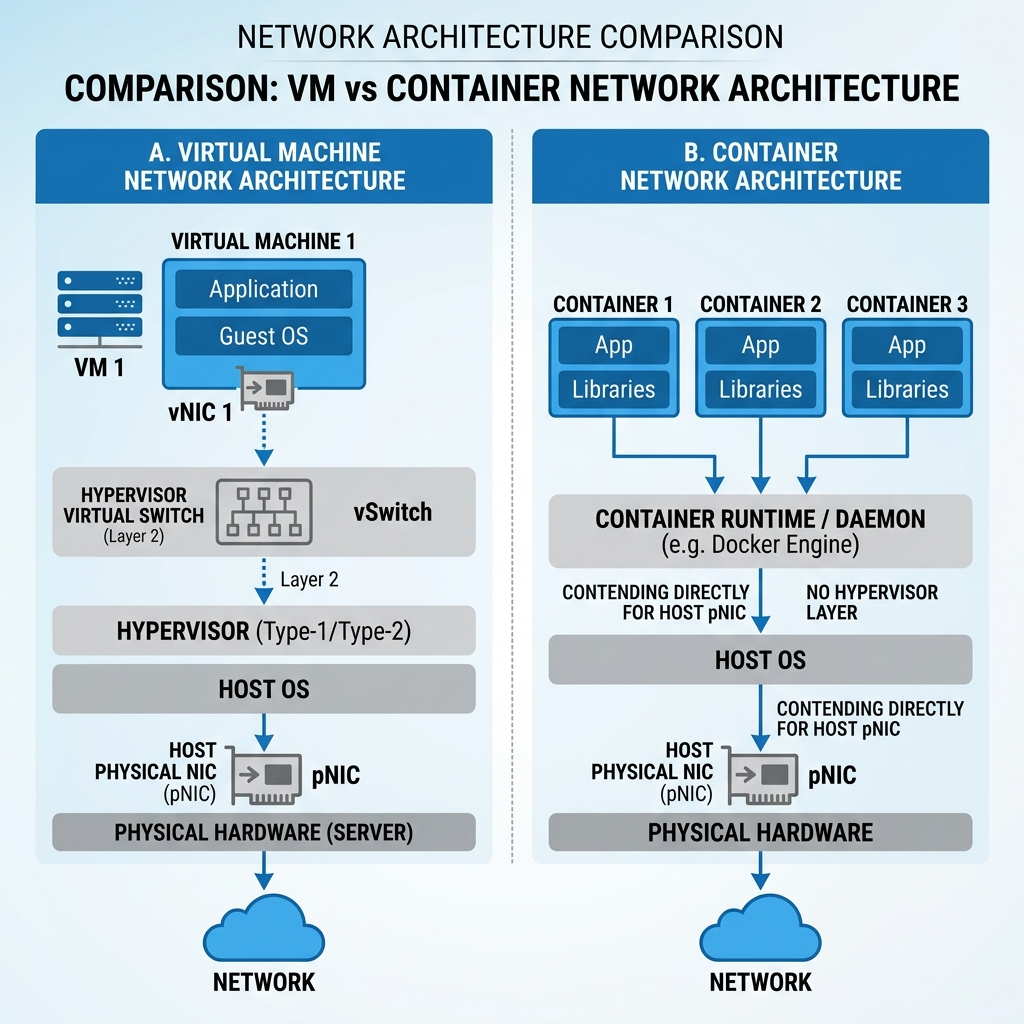
\includegraphics[width=0.8\textwidth]{images/container_vm_network.png}
    \caption{Architettura di rete: astrazione vNIC (VM) vs contesa e NAT (Container).}
\end{figure}

L'integrazione di Container e Virtualizzazione è però lo standard: il cloud esegue spesso cluster Kubernetes composti da \textit{Worker node} che sono essi stessi macchine virtuali, combinando così la leggerezza e facilità di deployment del container con il robusto isolamento hardware (evitando container escape) della VM.
